%%%%%%%%%%%%%%%%%%%%%%%%%%%%%%%%%%%%%%%%%
% Short Sectioned Assignment
% LaTeX Template
% Version 1.0 (5/5/12)
%
% This template has been downloaded from:
% http://www.LaTeXTemplates.com
%
% Original author:
% Frits Wenneker (http://www.howtotex.com)
%
% License:
% CC BY-NC-SA 3.0 (http://creativecommons.org/licenses/by-nc-sa/3.0/)
%
%%%%%%%%%%%%%%%%%%%%%%%%%%%%%%%%%%%%%%%%%

%----------------------------------------------------------------------------------------
%   PACKAGES AND OTHER DOCUMENT CONFIGURATIONS
%----------------------------------------------------------------------------------------

\documentclass[paper=a4, fontsize=11pt]{scrartcl} % A4 paper and 11pt font size

\usepackage[T1]{fontenc} % Use 8-bit encoding that has 256 glyphs
% \usepackage{fourier} % Use the Adobe Utopia font for the document - comment this line to return to the LaTeX default
\usepackage[english]{babel} % English language/hyphenation
\usepackage{amsmath,amsfonts,amsthm} % Math packages
\usepackage{spverbatim}
\usepackage{lipsum} % Used for inserting dummy 'Lorem ipsum' text into the template

\usepackage{sectsty} % Allows customizing section commands
\allsectionsfont{\centering \normalfont\scshape} % Make all sections centered, the default font and small caps

\usepackage{fancyhdr} % Custom headers and footers
\usepackage{graphicx}

\pagestyle{fancyplain} % Makes all pages in the document conform to the custom headers and footers
\fancyhead{} % No page header - if you want one, create it in the same way as the footers below
\fancyfoot[L]{} % Empty left footer
\fancyfoot[C]{} % Empty center footer
\fancyfoot[R]{\thepage} % Page numbering for right footer
\renewcommand{\headrulewidth}{0pt} % Remove header underlines
\renewcommand{\footrulewidth}{0pt} % Remove footer underlines
\setlength{\headheight}{13.6pt} % Customize the height of the header

\numberwithin{equation}{section} % Number equations within sections (i.e. 1.1, 1.2, 2.1, 2.2 instead of 1, 2, 3, 4)
\numberwithin{figure}{section} % Number figures within sections (i.e. 1.1, 1.2, 2.1, 2.2 instead of 1, 2, 3, 4)
\numberwithin{table}{section} % Number tables within sections (i.e. 1.1, 1.2, 2.1, 2.2 instead of 1, 2, 3, 4)

\setlength\parindent{0pt} % Removes all indentation from paragraphs - comment this line for an assignment with lots of text

%----------------------------------------------------------------------------------------
%   TITLE SECTION
%----------------------------------------------------------------------------------------

\newcommand{\horrule}[1]{\rule{\linewidth}{#1}} % Create horizontal rule command with 1 argument of height

\title{ 
\normalfont \normalsize 
\textsc{Iran University of Science and Technology, Computer Department} \\ [25pt] % Your university, school and/or department name(s)
\horrule{0.5pt} \\[0.4cm] % Thin top horizontal rule
\huge NLP Homework 2, Part 4 \\ % The assignment title
\horrule{2pt} \\[0.5cm] % Thick bottom horizontal rule
}

\author{Vahid Kharazi} % Your name

\date{\normalsize\today} % Today's date or a custom date

\begin{document}

\maketitle % Print the title

%----------------------------------------------------------------------------------------
%   PROBLEM 1
%----------------------------------------------------------------------------------------

\section{Support Transposiotion}


\begin{flushleft}

Levenshtein edit distance algorithm can support insert, delete and substitution.
\end{flushleft}

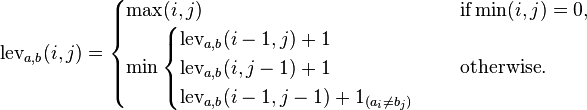
\includegraphics[scale=0.5]{lev.png}
\centering


\begin{flushleft}

By adding a simple rule after above equation, it can support transposition:

\end{flushleft}

\begin{spverbatim}
D[i][j] = min(D[i][j], D[i-2][j-1]) + cost  if(a[i-1]==b[j-2] and a[i-2]==b[j-1])

\end{spverbatim}

\begin{flushleft}
For the space complexity we need to store a $n*m$ matrix($O(nm)$). We add an operation(check, minimum and update) after basic Levenshtein algorithm. since we have direct access to matrix we don't have any change in time complexity($O(nm)$).

\end{flushleft}
\begin{flushleft}
There is three possible minimum edit distance:
\begin{enumerate}
\item If we can convert $a[1:i]$ to $b[1:j-1]$ by $k$ operation, so we will can simply convert it to $b[1:j]$ with $k + 1$ operations.
\item If we can convert $a[1:i-1]$ to $b[1:j]$ by $k$ operation, so we will can do it on $a[1:i-1]$ and them delete $a[i]$($k+1$ operations, delete is one).
\item If we can convert $a[1:i-1]$ to $b[1:j-1]$ by $k$ operation, so we will can do substitute $a[1:i]$ to $b[1:j]$($k+2$ operations, 2 is cost of substitution).
\end{enumerate}
For the added rule we have:
\begin{enumerate}
\item If we can convert $a[1:i-1]$ to $b[1:j-2]$ or $a[1:i-2]$ to $b[1:j-1]$ by $k$ operation, so we can do it with two substitution(cost of transposition).
\end{enumerate}
\end{flushleft}
\begin{flushleft}

The numbers of operation to convert $a[1:1-m]$ to $b[1:n-1]$. so we can say $D[m][n]$ is the final result.
\end{flushleft}

\end{document}